\section{Angular distribution of microwaves} \label{sec:Angular}

To examine the angular distribution of microwaves, the transmitter was placed on a goniometertable, such that the horn is located approximately at the pivot point.
The angular distribution was measured to both sides $\pm 90^\circ$ in equidistand steps. The measurements are done with a photo diode that is connected to an
Agilent 34402A. The measured intensity was normalized to 1 for $\theta = 0^\circ$ and is shown in fig. \ref{fig:angular}. The density of measured points around
$\theta = 0^\circ$ is quite low, which is not ideal. One should see the symmetry around the 0-point, but with our measurements, one can only guess it.\\
Nevertheless was the angle stretch of the radiation quantified by calculating the halfangle $\theta_H$ where the full width at half maximum lies. \\
\begin{equation}
    \theta_H = (28.4 \pm 2.5)^\circ
\end{equation}
\noindent
As expected due to the transmitter being a horn antenna, this confirms that the microwave radiation is pointed towards the $0^\circ$ direction.

\begin{figure}
\centering
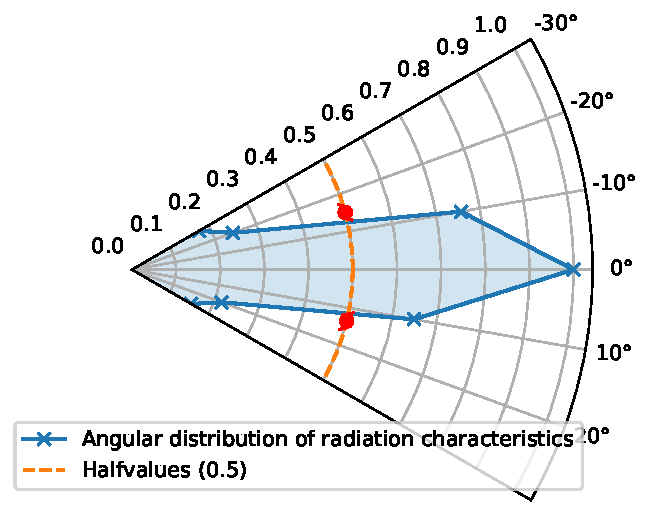
\includegraphics[width=0.5\textwidth]{../Images/Winkelverteilung_Polar.pdf}
\caption{Measured voltage within the relevant angular range normalized to 1 in dependence of the angle $\theta$. The left and right full width at half maximum are marked.}
\label{fig:angular}
\end{figure}